\section{System Overview}
Here is an image 
\begin{center}
		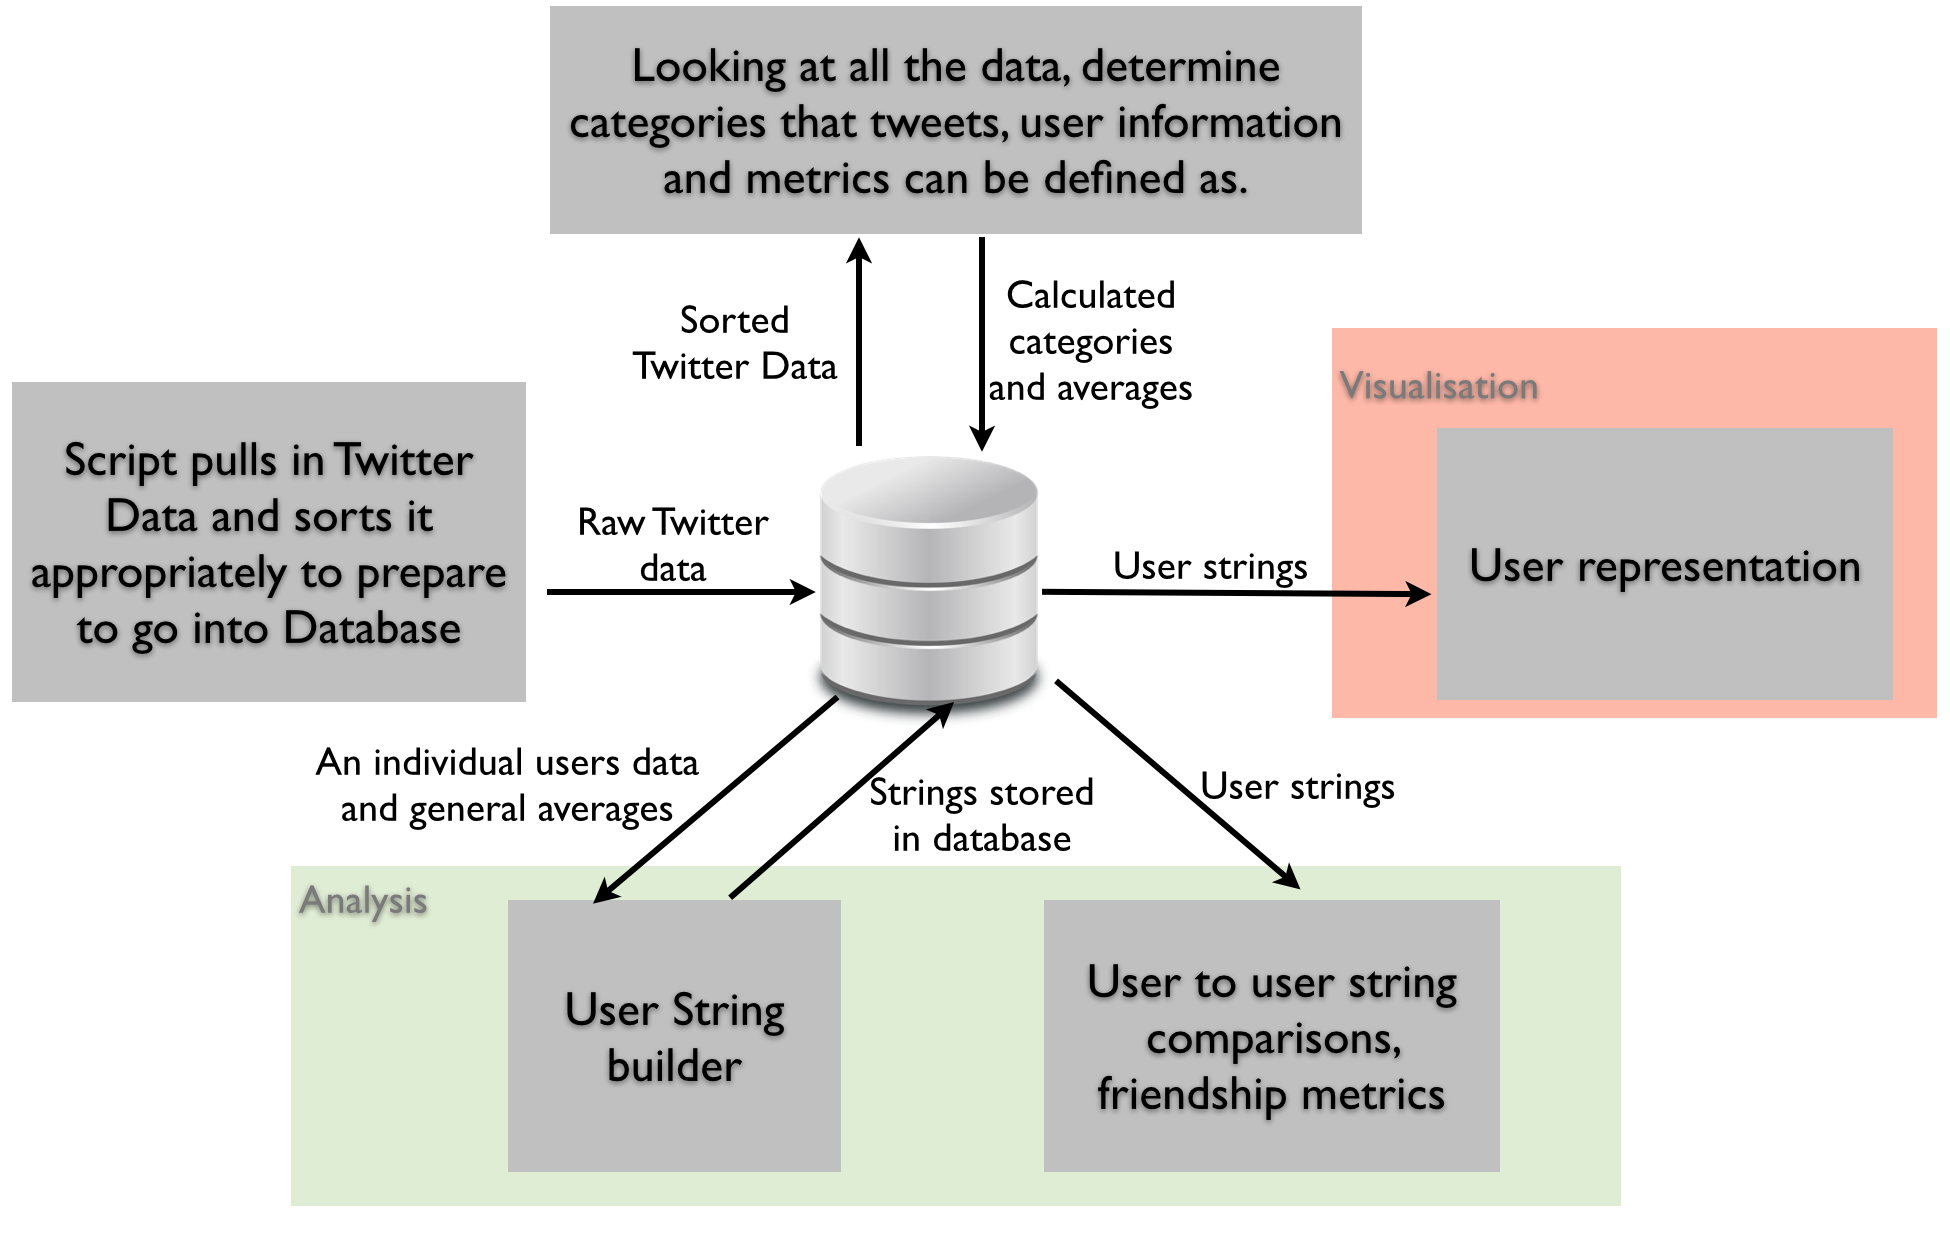
\includegraphics[scale = 0.55]{./images/architecture.png}
\end{center}
\section{Data Collection}
The first engine in the system is the data collection. Open source data sets are limited and not necessarily contianing relevant data, as well as possibly being biased towards certain topics, users or geographical locations, the need to produce a system which colleted data more relevant to this project was developed. 

\subsection{Database Design}
%Put schema in appendix!!!!
The idea of the Semantic Web is to give meaning to data, and in the case of Twitter this does not just mean the text in a users tweets. To understand more about a user, we can exploit information on Twitter:
\begin{itemize}
\item {\bf Tweets} - useful after having undergone analysis to extract meaning on interests and sentiment towards them. 
\item {\bf Following} - the types of people a user follows will indicate what they are interested in reading about
\item {\bf Followed By} - this is an indication of what they often tweet about. What is important to them that they feell should be expressed
\item {\bf Numerical Data} - such as how many friends and followers a user has. If very few they might be a Twitter sheep. 
\item {\bf Favourites and Retweets} - Giving stronger sentiment to the favourited tweets because they were found particularly important by the user. Or if a user has tweeted a particularly popular tweet then maybe they are more of an authority on this area. 
\item {\bf Hashtags} - used for emphasis on the object(?) of the conversation. Might give the topic more relavance to the user.
\end{itemize}
Hundreads of thousands of tweets are stored in the database and so an efficient schema needed to be designed in order to optimise space. This was done by only storing the text of the tweet once with details about it, such as how many times it was retweeted or favourited, by who it was made and it's ID. Then any retweet could simply reference the tweet ID in a separate table.
The database needed to be normalised for references. Tweets split into the tweet and it's details. Then a separate table for the users and referencing which tweets they said from the tweet table. 

\subsection{Unbiased Sampling of Twitter}
The graph that was being sampled consisted of nodes which were users and edges between them which indicated one relationship of either following or being followed by. When travelling between nodes it therefore makes the more popular users of Twitter much more likely to be visited repeatedly. It is important to note that if a user is popular and we would like to understand them better to see why they are so popular as this is useful information on what other users are interested in, but not in excess. Visiting many other users that have limited connections is also important. Therefore we can apply what is called the Metropolis-Hastings Random Walk algorithm to try and collect an unbiased sample of Twitter, where we are avoiding the bias of frequently visiting popular Twitter users.

\section{Analysis}
blah